\documentclass[12pt]{article}

\usepackage[utf8]{inputenc}
\usepackage[russian]{babel}
\usepackage[T2A]{fontenc}
\usepackage{textcomp}
\usepackage{a4wide}
\usepackage{amsmath, amssymb}
\usepackage{graphicx}
\usepackage{wrapfig}
\usepackage{caption}
\usepackage{subfig}
\usepackage{listings}
\usepackage{hyperref}
% \usepackage{fontspec}
\usepackage{pgfplots}
\usepackage{tikz}
\usepackage{amsthm}
\usepackage{pgf,pgfarrows,pgfnodes}
\usepackage{pgf}


\begin{document}
	
\renewcommand{\contentsname}{\centerline{\bf Contents}}
\renewcommand{\figurename}{Fig.}
\renewcommand{\refname}{\centerline{\bf Literature}}

\newcommand{\GP}{\mathcal{GP}}
\newcommand{\E}{\mathbb{E}}
\newcommand{\R}{\mathbb{R}}
\newcommand{\N}{\mathcal{N}}
\newcommand{\bigO}{\mathcal{O}}
\newcommand{\cov}{\mbox{cov}}
\newcommand{\Nystrom}{Nystr\"{o}m }
\newcommand{\KL}[2]{\mbox{KL}\left(#1\mbox{ || }#2\right)}
\newcommand{\tr}{\mbox{tr}}
\newcommand{\derivative}[2]{\frac{\partial #1}{\partial #2}}
\newcommand{\sndderivative}[3]{\frac{\partial^2 #1}{\partial #2 \partial #3}}

\newlength{\arrayrulewidthOriginal}
\newcommand{\Cline}[2]{%
  \noalign{\global\setlength{\arrayrulewidthOriginal}{\arrayrulewidth}}%
  \noalign{\global\setlength{\arrayrulewidth}{#1}}\cline{#2}%
  \noalign{\global\setlength{\arrayrulewidth}{\arrayrulewidthOriginal}}}

\newtheorem{definition}{Definition}
\newtheorem{theorem}{Theorem}


\begin{titlepage}
  \centering
  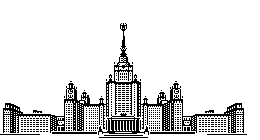
\includegraphics{pictures/msu.jpg}\par\vspace{1cm}
  {\scshape lomonosov Moscow State University\\ faculty of computational mathematics and cybernetics\\ chair of mathematical methods of forecasting \par}
  \vspace{2cm}
  {\scshape\large Izmailov Pavel\par}
  \vspace{1cm}
  {\LARGE\bfseries Gaussian Processes for Machine Learning\par}
  \vspace{1.5cm}
  {\scshape COURSE WORK\par}
  \vfill

  \raggedleft
  
  {\bf Scientific advisors:}\par
  % д.ф-м.н., профессор\par
  D. P. Vetrov\\
  D. A. Kropotov
  
  \vfill
  {\center\large Moscow, 2016\par}
\end{titlepage}

\pagebreak
\section{Introduction}
	
	Consider the following definition
	\begin{definition}
		A Gaussian process is a collection of random variables, any finite number of which have a joint Gaussian distribution.
	\end{definition}
	A Gaussian process is completely specified by it's mean function and covariance function. These functions are defined as follows
	\begin{definition}
		Let $f(x)$ be a real-valued Gaussian process. Then the functions
		$$m(x) = \E[f(x)],$$
		$$k(x, x') = \E[(f(x) - m(x)) (f(x') - m(x'))],$$
		are the mean function and the covariance function of the process $f$ respectively. 
	\end{definition}
	
	We will write the Gaussian process as $f(x) \sim \GP(m(x), k(x, x'))$.

\pagebreak
\begin{thebibliography}{99}
	
	\bibitem{GPinML}
	Rasmussen, C. E. and Williams, C. K. I. (2006). Gaussian Processes for Machine Learning. {\it MIT Press}.


	\bibitem{Titsias}
	Titsias M. K. (2009).  Variational Learning of Inducing Variables in Sparse Gaussian
	Processes.  In: {\it International Conference on Artificial Intelligence and Statistics}, pp.~567–574.

	\bibitem{BigData}
	Hensman J., Fusi N., Lawrence D. (2013).  Gaussian Processes for Big Data.  In: {\it Proceedings of the Twenty-Ninth Conference on Uncertainty in Artificial Intelligence}.

	\bibitem{SVIclassification}
	Hensman J., Matthews G., Ghahramani Z. (2015). Scalable Variational Gaussian Process Classification.  In: {\it Proceedings of the Eighteenth International Conference on Artificial Intelligence and Statistics}.


\end{thebibliography}	
\end{document}
